\section{Conclusiones y disponibilidad}\label{sec:conclusiones}

Este trabajo ha formalizado el modelo \textbf{SM-CFHR} (\textit{Structured Monotone Capacity-Factor Huber Regressor}), su análisis matemático y verificación formal en Lean~4, la evaluación OOF congelada sobre $28$ configuraciones (\texttt{v1.0.3}), la reconciliación inferencial y en factor de capacidad (\texttt{v2.0.0}) y el experimento controlado de equivalencia de representación y ablación factorial (\texttt{v3.0.0}).

En el plano teórico y formal, la normalización causal por capacidad vigente al origen ($24\,000\,C_{i,t}$) unifica objetivos diarios y acumulados eliminando la heterogeneidad de $39{,}6\times$ sin fuga temporal; asimismo, el programa convexo de Huber con regularización anisotrópica y cotas de no negatividad posee existencia global, unicidad de $\mathbf{w}^*$, unicidad condicional de $b^*$ y equivalencia KKT verificadas en Lean~4 (\texttt{v4.36.0}) sobre $\mathbb{R}$ (con demostración analítica de la cota espectral completa $L_J$ en el Material Suplementario, Sección~S1).

En el plano empírico, la evidencia combinada de las tres capas del estudio permite concluir con precisión:
\begin{enumerate}
    \item \textbf{La contribución principal demostrada es la representación causal en factor de capacidad y el protocolo multihorizonte sin fuga:} al equiparar la representación a factor de capacidad en \texttt{v3.0.0}, las siete familias evaluadas mejoran entre $-10{,}13\%$ y $-23{,}24\%$ en $\mathrm{MAE}_{\mathrm{CF,macro}}$ medio, y retirar dicha normalización degrada el error en $+25{,}86\%$ de media (hasta $+62{,}65\%$).
    \item \textbf{No se demuestra superioridad algorítmica universal de SM-CFHR frente a lineales regularizados en factor de capacidad:} bajo representación equiparada, \texttt{SM-CFHR} empata o queda a $+0{,}13\%$--$+1{,}58\%$ de \texttt{BayesianRidge-CF} y \texttt{ElasticNet-CF} en transferencia espaciotemporal (ganando solo en \texttt{RecGEFSv12\_ET\_7d} en Condición~A, $-0{,}56\%$, y en \texttt{D1\_ET\_5var} en Condición~B, $-0{,}09\%$) y pierde sistemáticamente en régimen intraplanta ($+3{,}23\%$ a $+16{,}24\%$).
    \item \textbf{Los componentes secundarios aportan beneficios acotados o dependientes del régimen:} las variables NWP ($+18{,}52\%$) y anomalías ($+5{,}61\%$) son determinantes; la configuración fija ($B=0$) supera a \texttt{HPO} ($B=25$) en $19/28$ escenarios con coste $59\times$ menor; y la pérdida de Huber protege frente a contaminación severa del objetivo ($10\%$) pero no ante apalancamiento en covariables. Permanece vigente \texttt{autorizacion\_alcance\_solar\_docente: false}.
\end{enumerate}

\subsection*{Disponibilidad de código y reproducibilidad}

El código fuente del estimador, el protocolo experimental, las pruebas automatizadas, la formalización en Lean~4 y el manuscrito están disponibles para reproducción computacional \cite{peng2011reproducible} en el repositorio oficial \url{https://github.com/KrissV89/sm-cfhr} (etiqueta de publicación \texttt{v1.0.3-polyform}, protocolo científico \texttt{v1.0.3}, con huella SHA-256 verificable del núcleo matemático). El software original se distribuye bajo la licencia \textbf{PolyForm Noncommercial~1.0.0}, que permite el uso gratuito para investigación académica, estudio y reproducción científica; todo uso comercial o con ánimo de lucro requiere licencia comercial aparte (\texttt{edmolinares@soulspacers.com}). Esta licencia cubre únicamente el código original: los datos externos de XM, Open-Meteo y Global Energy Monitor mantienen sus propias condiciones de uso (por su tamaño de $603{,}70$~MB sin comprimir y restricciones de redistribución se provee un flujo de importación local y verificación SHA-256; Figura~\ref{fig:pipeline_repro}), las dependencias de terceros conservan sus respectivas licencias y el presente manuscrito junto con sus figuras mantiene sus derechos académicos independientes.

\begin{figure}[!htbp]
\centering
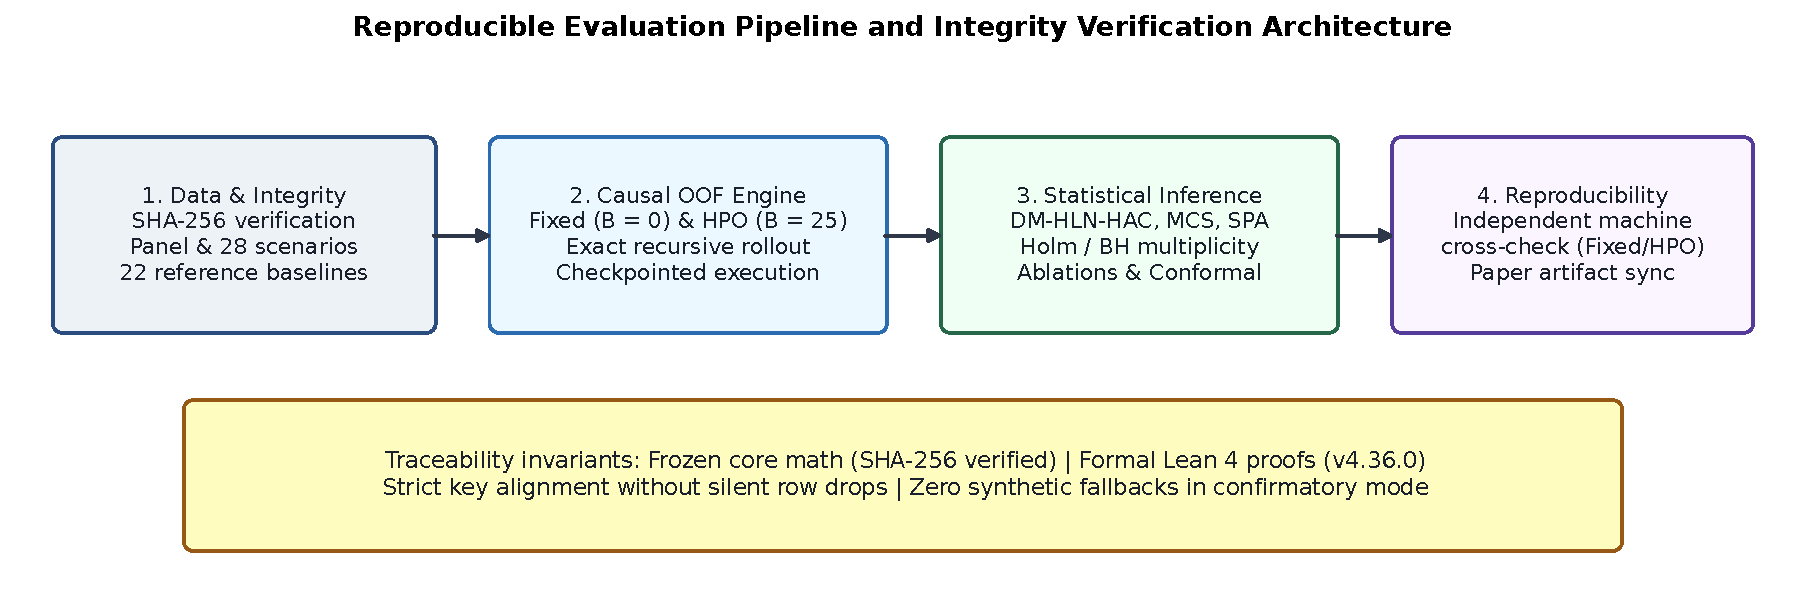
\includegraphics[width=0.98\textwidth]{figures/fig_pipeline_reproduccion.pdf}
\caption{Arquitectura de ejecución resumible, verificación de integridad mediante SHA-256 y comparación numérica entre máquinas independientes.}
\label{fig:pipeline_repro}
\end{figure}
